\documentclass{article}
\usepackage{graphicx} % Required for inserting images
\usepackage{titling}
\usepackage[lithuanian]{babel}
\usepackage{tocloft}
\usepackage{secdot} % uždeda tašką po skyriaus numerio
\usepackage{amsmath} % For math environments
\usepackage{amssymb} % For additional math symbols
\usepackage{hyperref} % For hyperlinks
\sectiondot{subsection} % uždeda tašką po poskyrio numerio
\usepackage{indentfirst} % atitraukia pirmą dokumento pastraipą
\renewcommand{\cftsecaftersnum}{.} % Uždeda tašką po skyriaus numerio turinyje
\renewcommand{\cftsubsecaftersnum}{.} % Uždeda tašką po poskyrio numerio turinyje

\setlength{\droptitle}{-2cm} % Adjusts the space before the title
\title{Prakinė informatika 11-12 užduotis}
\author{Karolis Paškevičius}
\date{2024-12-15}


\begin{document}

\maketitle

\section{Mūro dėsnis}
Mūro dėsnis (\textit{angl. Moore's law}) yra empiriškai pastebėta tendencija, kad tranzistorių skaičius integruotose mikroschemose dvigubėja vidutiniškai kas dvejus metus. Ši tendencija yra pavadinta Gordono Mūro (\textit{Gordon Moore}), \textit{Fairchild Semiconductor} ir \textit{Intel} įmonių vieno iš įkūrėjų, garbei. Jis 1965 metais pastebėjo, kad komponentų skaičius sudėtingose integruotose grandinėse dvigubėja vidutiniškai kas dvejus metus. Šis dėsnis galioja ir kompiuterių centriniams procesoriams (\textit{angl. central processing unit}).
\begin{figure}[h!]
    \raggedright
    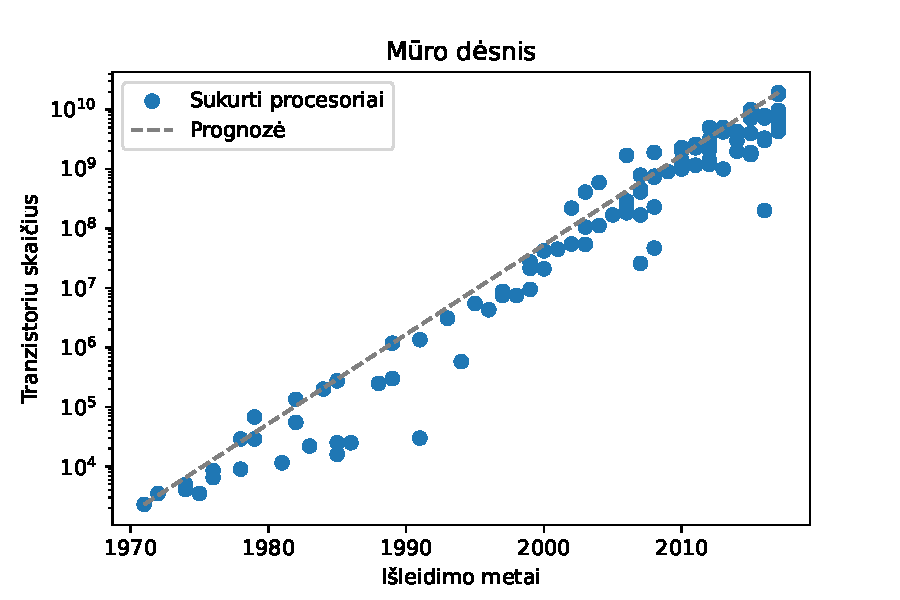
\includegraphics[width=\textwidth]{muro_desnis.pdf}
    \caption{Tranzistorių skaičiaus kompiuterių centriniuose procesoriuose priklausomybė nuo jų išleidimo metų (mėlyni taškai) ir prognozė pagal Mūro dėsnio formulę (pilka punktyrinė linija).}
    \label{fig:muro}
\end{figure}

Mūro dėsnis yra naudojamas puslaidininkų pramonėje ilgalaikių tikslų 
planavimui, todėl iš dalies tapo savaime išsipildančia pranašyste. Šis dėsnis stebimas ir kitoms kompiuterių dalims kaip operatyvinė atmintis (angl. \textit{random access memory}), skaitmeninių fotoparatų jutikliams.


\section{Pratybų užduotys}  % This will be numbered as "2"
Čia atliksime 12 užduotį

\subsection{Nurodomas poskyris} 
\label{subsec:nurodomas}  % Add a label for this subsection
Kaip referavome į \ref{subsec:nurodantis} poskyrį, lygiai taip pat galime referuoti ir į grafiką. Hiperbolių nubraižytų su Matplotlib pavyzdys yra \ref{fig:hiperbole} pav.

\begin{figure}[h!]
    \raggedright
    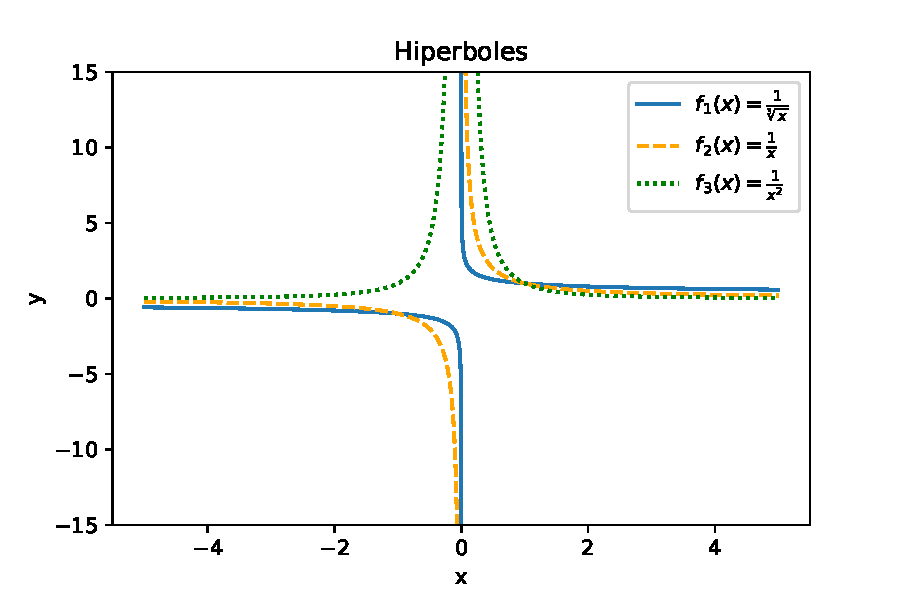
\includegraphics[width=\textwidth]{funk.pdf}
    \caption{Hiperbolių grafikai, nubraižyti su Matplotlib.}
    \label{fig:hiperbole}
\end{figure}

\pagebreak
\subsection{L\textsc{a}\TeX\ formulių pavyzdžiai}
Toliau užrašysime kelis formulių pavyzdžius.

Pirmųjų \( n \) natūraliųjų skaičių kvadratų suma:
\begin{equation}
    1^2 + 2^2 + 3^2 + \cdots + n^2 = \sum_{k=1}^{n} k^2 = \frac{1}{6} n (n+1)(2n+1)
    \label{eq:squaresum}
\end{equation}

Apibrėžtinio integralo pavyzdys:
\begin{equation}
    \int_{0}^{\infty} \frac{\sin x}{x} \, dx = \frac{\pi}{2}
    \label{eq:integral1}
\end{equation}

Eulerio lygtis:
\begin{equation}
    e^{i\phi} = \cos \phi + i \sin \phi
    \label{eq:euler2}
\end{equation}

Iš Eulerio lygties \eqref{eq:euler2} nesudėtinga išvesti Eulerio tapatybę:
\begin{equation}
    e^{i\pi} + 1 = 0
    \label{eq:euler1}
\end{equation}

Į formules taip pat galima referuoti: 
apibrėžtinio integralo pavyzdys yra \eqref{eq:integral1} formulėje,
Eulerio lygtis -- \eqref{eq:euler2} formulėje, 
o Eulerio tapatybė -- \eqref{eq:euler1} formulėje.

\subsection{Nurodantis poskyris}
\label{subsec:nurodantis}  % Add a label for this subsection
Šiame skyriuje nurodyta svarbi informacija.

\subsection{Nurodantis poskyris} 
Šiame skyriuje nurodyta kita informacija, papildomai žr. \ref{subsec:nurodantis} poskyrį.

\end{document}


\end{document}
